\documentclass[a4paper]{article}
%\documentclass{tuftebook}
\usepackage{amsthm}
\usepackage[many]{tcolorbox}

\makeatletter

\makeatletter

\def\renewtheorem#1{%
	\expandafter\let\csname#1\endcsname\relax
	\expandafter\let\csname c@#1\endcsname\relax
	\gdef\renewtheorem@envname{#1}
	\renewtheorem@secpar
}
\def\renewtheorem@secpar{\@ifnextchar[{\renewtheorem@numberedlike}{\renewtheorem@nonumberedlike}}
\def\renewtheorem@numberedlike[#1]#2{\newtheorem{\renewtheorem@envname}[#1]{#2}}
\def\renewtheorem@nonumberedlike#1{
	\def\renewtheorem@caption{#1}
	\edef\renewtheorem@nowithin{\noexpand\newtheorem{\renewtheorem@envname}{\renewtheorem@caption}}
	\renewtheorem@thirdpar
}
\def\renewtheorem@thirdpar{\@ifnextchar[{\renewtheorem@within}{\renewtheorem@nowithin}}
\def\renewtheorem@within[#1]{\renewtheorem@nowithin[#1]}

\makeatother

%%%%%%%%%%%%%%%%%%%%
% New environments %
%%%%%%%%%%%%%%%%%%%%

\makeatother
%\mdfsetup{skipabove=1em,skipbelow=0em}

\tcbuselibrary{skins}

% Color definitions

\definecolor{proofcolor}{RGB}{0,0,0}

% Dark orange and Dark Red rgb
\definecolor{theorembordercolor}{RGB}{151, 63, 5}
\definecolor{theorembackgroundcolor}{RGB}{248, 241, 234}

\definecolor{examplebordercolor}{RGB}{0, 110, 184}
\definecolor{examplebackgroundcolor}{RGB}{240, 244, 250}

\definecolor{definitionbordercolor}{RGB}{0, 150, 85}
\definecolor{definitionbackgroundcolor}{RGB}{239, 247, 243}

\definecolor{propertybordercolor}{RGB}{128, 0, 128}
\definecolor{propertybackgroundcolor}{RGB}{255, 240, 255}

\definecolor{formulabordercolor}{RGB}{0, 0, 0}
\definecolor{formulabackgroundcolor}{RGB}{230, 229, 245}

\newtheoremstyle{theorem}
{0pt}{0pt}{\normalfont}{0pt}
{}{\;}{0.25em}
{{\sffamily\bfseries\color{theorembordercolor}\thmname{#1}~\thmnumber{\textup{#2}}.}
	\thmnote{\normalfont\color{black}~(#3)}}

\newtheoremstyle{definition}
{0pt}{0pt}{\normalfont}{0pt}
{}{\;}{0.25em}
{{\sffamily\bfseries\color{definitionbordercolor}\thmname{#1}~\thmnumber{\textup{#2}}.}
	\thmnote{\normalfont\color{black}~(#3)}}

\newtheoremstyle{example}
{0pt}{0pt}{\normalfont}{0pt}
{}{\;}{0.25em}
{{\sffamily\bfseries\color{examplebordercolor}\thmname{#1}.}
	\thmnote{\normalfont\color{black}~(#3)}}

\newtheoremstyle{property}
{0pt}{0pt}{\normalfont}{0pt}
{}{\;}{0.25em}
{{\sffamily\bfseries\color{propertybordercolor}\thmname{#1}~\thmnumber{\textup{#2}}.}
	\thmnote{\normalfont\color{black}~(#3)}}

\newtheoremstyle{formula}
{0pt}{0pt}{\normalfont}{0pt}
{}{\;}{0.25em}
{{\sffamily\bfseries\color{formulabordercolor}\thmname{#1}~\thmnumber{\textup{#2}}.}
	\thmnote{\normalfont\color{black}~(#3)}}

%%%%%%%%%%%%%%%%%%%%%%%%
% Theorem Environments %
%%%%%%%%%%%%%%%%%%%%%%%%

\theoremstyle{theorem}

\newtheorem{theorem}{Theorem}
\newtheorem{postulate}{Postulate}
\newtheorem{conjecture}{Conjecture}
\newtheorem{corollary}{Corollary}
\newtheorem{lemma}{Lemma}
\newtheorem{conclusion}{Conclusion}

\tcolorboxenvironment{theorem}{
	enhanced jigsaw, pad at break*=1mm, breakable,
	left=4mm, right=4mm, top=1mm, bottom=1mm,
	colback=theorembackgroundcolor, boxrule=0pt, frame hidden,
	borderline west={0.5mm}{0mm}{theorembordercolor}, arc=.5mm
}
\tcolorboxenvironment{postulate}{
	enhanced jigsaw, pad at break*=1mm, breakable,
	left=4mm, right=4mm, top=1mm, bottom=1mm,
	colback=theorembackgroundcolor, boxrule=0pt, frame hidden,
	borderline west={0.5mm}{0mm}{theorembordercolor}, arc=.5mm
}
\tcolorboxenvironment{conjecture}{
	enhanced jigsaw, pad at break*=1mm, breakable,
	left=4mm, right=4mm, top=1mm, bottom=1mm,
	colback=theorembackgroundcolor, boxrule=0pt, frame hidden,
	borderline west={0.5mm}{0mm}{theorembordercolor}, arc=.5mm
}
\tcolorboxenvironment{corollary}{
	enhanced jigsaw, pad at break*=1mm, breakable,
	left=4mm, right=4mm, top=1mm, bottom=1mm,
	colback=theorembackgroundcolor, boxrule=0pt, frame hidden,
	borderline west={0.5mm}{0mm}{theorembordercolor}, arc=.5mm
}
\tcolorboxenvironment{lemma}{
	enhanced jigsaw, pad at break*=1mm, breakable,
	left=4mm, right=4mm, top=1mm, bottom=1mm,
	colback=theorembackgroundcolor, boxrule=0pt, frame hidden,
	borderline west={0.5mm}{0mm}{theorembordercolor}, arc=.5mm
}
\tcolorboxenvironment{conclusion}{
	enhanced jigsaw, pad at break*=1mm, breakable,
	left=4mm, right=4mm, top=1mm, bottom=1mm,
	colback=theorembackgroundcolor, boxrule=0pt, frame hidden,
	borderline west={0.5mm}{0mm}{theorembordercolor}, arc=.5mm
}

%%%%%%%%%%%%%%%%%%%%%%%%%%%
% Definition Environments %
%%%%%%%%%%%%%%%%%%%%%%%%%%%

\theoremstyle{definition}
\newtheorem{definition}{Definition}
\newtheorem{review}{Review}

\tcolorboxenvironment{definition}{
	enhanced jigsaw, pad at break*=1mm, breakable,
	left=4mm, right=4mm, top=1mm, bottom=1mm,
	colback=definitionbackgroundcolor, boxrule=0pt, frame hidden,
	borderline west={0.5mm}{0mm}{definitionbordercolor}, arc=.5mm
}
\tcolorboxenvironment{review}{
	enhanced jigsaw, pad at break*=1mm, breakable,
	left=4mm, right=4mm, top=1mm, bottom=1mm,
	colback=definitionbackgroundcolor, boxrule=0pt, frame hidden,
	borderline west={0.5mm}{0mm}{definitionbordercolor}, arc=.5mm
}


%%%%%%%%%%%%%%%%%%%%%%%%
% Example Environments %
%%%%%%%%%%%%%%%%%%%%%%%%

\theoremstyle{example}
\newtheorem*{example}{Example}
\newtheorem*{remark}{Remark}
\newtheorem*{note}{Note}

\tcolorboxenvironment{example}{
	enhanced jigsaw, pad at break*=1mm, breakable,
	left=4mm, right=4mm, top=1mm, bottom=1mm,
	colback=examplebackgroundcolor, boxrule=0pt, frame hidden,
	borderline west={0.5mm}{0mm}{examplebordercolor}, arc=.5mm
}
\tcolorboxenvironment{remark}{
	enhanced jigsaw, pad at break*=1mm, breakable,
	left=4mm, right=4mm, top=1mm, bottom=1mm,
	colback=white, boxrule=0pt, frame hidden,
	borderline west={0.5mm}{0mm}{examplebordercolor}, arc=.5mm
}
\tcolorboxenvironment{note}{
	enhanced jigsaw, pad at break*=1mm, breakable,
	left=4mm, right=4mm, top=1mm, bottom=1mm,
	colback=white, boxrule=0pt, frame hidden,
	borderline west={0.5mm}{0mm}{examplebordercolor}, arc=.5mm
}


%%%%%%%%%%%%%%%%%%%%%%%%%
% Property Environments %
%%%%%%%%%%%%%%%%%%%%%%%%%

\theoremstyle{property}
\newtheorem{property}{Property}
\newtheorem{proposition}{Proposition}

\tcolorboxenvironment{property}{
	enhanced jigsaw, pad at break*=1mm, breakable,
	left=4mm, right=4mm, top=1mm, bottom=1mm,
	colback=propertybackgroundcolor, boxrule=0pt, frame hidden,
	borderline west={0.5mm}{0mm}{propertybordercolor}, arc=.5mm
}
\tcolorboxenvironment{proposition}{
	enhanced jigsaw, pad at break*=1mm, breakable,
	left=4mm, right=4mm, top=1mm, bottom=1mm,
	colback=propertybackgroundcolor, boxrule=0pt, frame hidden,
	borderline west={0.5mm}{0mm}{propertybordercolor}, arc=.5mm
}

%%%%%%%%%%%%
% Formula %
%%%%%%%%%%%%

\theoremstyle{formula}
\newtheorem{formula}{Formula}

\tcolorboxenvironment{formula}{
	enhanced jigsaw, pad at break*=1mm, breakable,
	left=4mm, right=4mm, top=1mm, bottom=1mm,
	colback=formulabackgroundcolor, boxrule=0pt, frame hidden,
	borderline west={0.5mm}{0mm}{formulabordercolor}, arc=.5mm
}

%%%%%%%%%
% Proof %
%%%%%%%%%

% These patches must be placed after \tcolorboxenvironment !
\AddToHook{env/theorem/after}{\colorlet{proofcolor}{theorembordercolor}}
\AddToHook{env/postulate/after}{\colorlet{proofcolor}{theorembordercolor}}
\AddToHook{env/conjecture/after}{\colorlet{proofcolor}{theorembordercolor}}
\AddToHook{env/corollary/after}{\colorlet{proofcolor}{theorembordercolor}}
\AddToHook{env/lemma/after}{\colorlet{proofcolor}{theorembordercolor}}
\AddToHook{env/conclusion/after}{\colorlet{proofcolor}{theorembordercolor}}

\AddToHook{env/definition/after}{\colorlet{proofcolor}{definitionbordercolor}}
\AddToHook{env/review/after}{\colorlet{proofcolor}{definitionbordercolor}}

\AddToHook{env/example/after}{\colorlet{proofcolor}{examplebordercolor}}
\AddToHook{env/remark/after}{\colorlet{proofcolor}{examplebordercolor}}
\AddToHook{env/note/after}{\colorlet{proofcolor}{examplebordercolor}}

\AddToHook{env/property/after}{\colorlet{proofcolor}{propertybordercolor}}
\AddToHook{env/proposition/after}{\colorlet{proofcolor}{propertybordercolor}}

\AddToHook{env/formula/after}{\colorlet{proofcolor}{formulabordercolor}}

\renewcommand{\qedsymbol}{Q.E.D.}
\let\qedsymbolMyOriginal\qedsymbol
\renewcommand{\qedsymbol}{
	\color{proofcolor}\qedsymbolMyOriginal
}

\newtheoremstyle{proof}
{0pt}{0pt}{\normalfont}{0pt}
{}{\;}{0.25em}
{{\sffamily\bfseries\color{proofcolor}\thmname{#1}.}
	\thmnote{\normalfont\color{black}~(\textit{#3})}}

\theoremstyle{proof}
\renewtheorem{proof}{Proof}

\tcolorboxenvironment{proof}{
	enhanced jigsaw, pad at break*=1mm, breakable,
	left=4mm, right=4mm, top=1mm, bottom=1mm,
	colback=white, boxrule=0pt, frame hidden,
	borderline west={0.5mm}{0mm}{proofcolor}, arc=.5mm
}

\newenvironment{info}{\begin{tcolorbox}[
		arc=0mm,
		colback=white,
		colframe=gray,
		title=Info,
		fonttitle=\sffamily,
		breakable
		]}{\end{tcolorbox}}
\newenvironment{terminology}{\begin{tcolorbox}[
		arc=0mm,
		colback=white,
		colframe=green!60!black,
		title=Terminology,
		fonttitle=\sffamily,
		breakable
		]}{\end{tcolorbox}}
\newenvironment{warning}{\begin{tcolorbox}[
		arc=0mm,
		colback=white,
		colframe=red,
		title=Warning,
		fonttitle=\sffamily,
		breakable
		]}{\end{tcolorbox}}
\newenvironment{caution}{\begin{tcolorbox}[
		arc=0mm,
		colback=white,
		colframe=yellow,
		title=Caution,
		fonttitle=\sffamily,
		breakable
		]}{\end{tcolorbox}}
\graphicspath{{images/}}

\date{}
\title{\flushleft \textbf{K-Cell}}

\begin{document}
	\maketitle
	Last time, we talked about:
	\begin{enumerate}
		\item Compact $\implies$ closed and bounded.
		\item Closed subsets of compact sets are compact.
		\item If $\ocover{K}$ is compact and every finite intersection is nonempty, then $\bigcap \limits_{\alpha \in \Lambda} K_\alpha \not = \emptyset$
	\end{enumerate}
	
	\begin{corollary}
		If $K_1 \supseteq K_2 \supseteq K_3 \supseteq K_4 \supseteq ...$ is a sequence of nonempty compact sets, then $\bigcap \limits_{i=1}^\infty K_n$ is nonempty.
	\end{corollary}
	
	\begin{property}[Nested Interval Property]
		If $I_n=[a_n,b_n]$ is a sequence of closed intervals in $\R$ \st $I_1 \supseteq I_2 \supseteq I_3 \supseteq ...,$ then $\bigcap \limits_{n=1}^\infty I_n$ is nonempty.
	\end{property}
	
	In $\R ^k$, closed and bounded implies compactness.
	
	\begin{definition}[K-Cell]
		The set $I = [a_1,b_1 ] \times ... \times [a_k, b_k]$ is called a k-cell in $\R ^k$.
	\end{definition}
	
	For example, $I=[a_1, b_1] \times [a_2, b_2]$ in $\R ^2$ \\:
	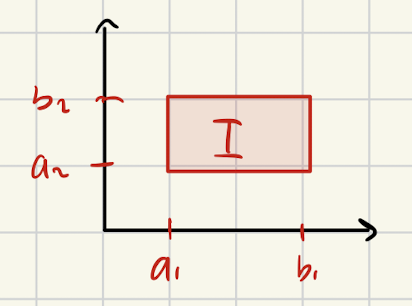
\includegraphics[width= 100pt, center]{K.png}
	
	\begin{theorem} (Nested Cell Property)
		If $I_1 \supseteq I_2 \supseteq I_3 \supseteq ...$ is a nested sequence of k-cells, then $\bigcap \limits_{n=1}^\infty I_n \not = \emptyset$.
	\end{theorem}
	\begin{proof}
		For each $n\in \N$, let
		$$I_n = [a_1 ^{(1)}, b_1 ^{(1)}] \times ... \times [a_k ^{(k)}, b_k ^{(k)}].$$
		Also, let
		$$ \forall n \in \N ~~\forall 1 \leq i \leq k ~~A_i ^{(i)} = [a_i ^{(n)}, b_i^{(n)}].$$
		So, 
		$$ \forall n \in \N ~~I_n = A_1^{(n)} \times ... \times A_k ^{(n)}.$$
		Since for each $n \in \N$, $I_n \supseteq I_{n+1},$ we have
		$$\forall 1 \leq i \leq k ~~ A_i ^{(n)} \supseteq A_i^{(n+1)}$$
		That is,
		\begin{align*}
			I_1 &= A_1^{(1)} \times ... \times A_k ^{(1)} \\
			I_2 &= A_2 ^{(2)} \times ... \times A_k^{(2)} \\
			\vdots \\
			I_n &= A_n^{(1)} \times ... \times A_n^{(n)} \\
			\vdots
		\end{align*}
		Hence, it follows from the nested interval property that
		$$\exists x_1 \in \bigcap \limits_{n=1}^\infty A_1^{(n)}, \exists x_2 \in \bigcap \limits_{n=1}^\infty A_2^{(n)}, ... \exists x_k \in \bigcap \limits{n=1}^{\infty} A_k ^{(n)}$$
		Thus,
		\begin{align*}
			(x_1,...,x_n) &\in \left[\bigcap \limits_{n=1}^\infty A_1^{(n)}\right] \times \left[\bigcap \limits_{n=1}^\infty A_2^{(n)}\right] \times... \times \left[\bigcap \limits_{n=1}^\infty A_k^{(n)}\right] \\
			&\subseteq \bigcap \limits_{n=1}^\infty \left[A_1^{(1)} \times ... \times A_k^{(n)}\right] \\
			&= \bigcap \limits_{n=1}^\infty I_n
		\end{align*}
		So, $\bigcap \limits_{n=1}^\infty I_n \not = \emptyset.$ \qed
	\end{proof}
	
	\begin{theorem}
		Every k-cell in $\R ^k$ is compact.
	\end{theorem}

	\begin{proof}
		Here we will prove the claim for 2-cells. The proof for a general k-cell is completely analogous.
		Let $I = [a_1,b_1] \times [a_2,b_2]$ be a 2-cell. Let $\varrow{a}=(a_1,a_2)$ and $\varrow{b}=(b_1,b_2)$.
		Let $\delta = d(\varrow{a}, \varrow{b})= ||\varrow{a} - \varrow{b}||_2 = sqrt{(a_1-b_1)^2+(a_2-b_2)^2}.$
		Noe that if $\varrow{x}=(x_1,x_2)$ and $\varrow{y}=(y_1,y_2)$ are any two points in I, then
		$$\begin{cases}
			x_1,y_1 \in [a_1,b_1] &\implies |x_1 - y_1| \leq |b_1 - a_1| \\
			x_2,y_2 \in [a_2,b_2] &\implies |x_2 - y_2| \leq |b_2 - a_2| \\
		\end{cases}
		\implies \sqrt{|x_1-y_1|^2+|x_2-y_2|^2} \leq \sqrt{|a_1-b_1|^2+|a_2-b_2|^2} = \delta$$
		So, $$d(\varrow{x}, \varrow{y}) \leq \delta.$$
		Let's assume for contradiction that $I$ is not compact. So, there exists an open cover $\ocover{G}$ of $I$ that does not have a finite subcover.
		For each $1 \leq i \leq 2$, divide $[a_i, b_i]$ into two subintervals of equal length:
		$$c_i= \frac{a_i + b_i}{2}, ~~ [a_i,b_i]=[a_i, c_i] \cup [c_i, b_i]$$
		These subintervals determine four 2-cells. There is at least one of these four 2-cells that is not covered by any finite subcollection of $\ocover{G}$.
		Let's call it $I_1$. Notice that
		$$\forall \varrow{x}, \varrow{y} \in I_1 ~~ ||\varrow{x}, \varrow{y}||_2 \leq \frac{\delta}{2}.$$
		Now, subdivide $I_1$ into four 2-cells and continue this process. We will obtain a sequence of 2-cells
		$$I_1, I_2, I_3, ... $$
		such that
		\begin{align*}
			&(i) I \supseteq I_1 \supseteq I_2 \supseteq ... \\
			&(ii) \forall \varrow{x}, \varrow{y} \in I_n ~~ ||\varrow{x}-\varrow{y}|| \leq \frac{\delta}{2^n} \\
			&(iii) \forall n \in \N, I_n \text{ cannot be covered by a finite subcollection of } \ocover{G}.
		\end{align*}
		By the nested cell property,
		$$\exists \varrow{x}^* \in I\cap I_1 \cap I_2 \cap...$$
		In particular,
		$$\varrow{x}^* \in I \subseteq \ocover{G} \implies \exists \alpha_0 \st \varrow{x}^* \in G_{\alpha_0}$$
		We have
		$$\begin{rcases}
			\varrow{x}^* \in G_{\alpha_0} \\
			G_{\alpha_0} \text{ is open}
		\end{rcases}
		\implies \exists r > 0 \st N_r(\varrow{x}^*) \subseteq G_{\alpha_0}$$
		Choose $n\in \N \st \frac{\delta}{2^n} < r.$ We claim that $I_n \in \nbhd{r}{\varrow{x}^*}.$ Indeed,
		suppose $\varrow{y}\in I_n$, we have $$\begin{cases}
			\varrow{y}\in I_n \\
			\varrow{x}^* \in I_n
		\end{cases}$$
		so $||\varrow{y} - \varrow{x}|| \leq \frac{\delta}{2^n} < r.$ Hence $\varrow{y} \in \nbhd{r}{\varrow{x}^*}.$ We have
		$$\begin{rcases}
			I_n \subseteq \nbhd{r}{\varrow{x}^*} \\
			\nbhd{r}{\varrow{x}^*} \subseteq G_{\alpha_0}
		\end{rcases}
		\implies I_n \subseteq G_{\alpha_0}$$
		This contradicts $(iii)$. \qed
	\end{proof}

	\begin{theorem}[Heine-Borel Theorem]
		Let $E\subseteq \R^k$. The following statements are equivalent:
		\begin{enumerate}
			\item $E$ is closed and bounded.
			\item $E$ is compact.
			\item Every infinite subset of $E$ has a limit point in $E$.
		\end{enumerate}
	\end{theorem}
	\begin{proof}
		We will show $1. \implies 2. \implies 3. \implies 1.$ \\
		$1. \implies 2.:$ Suppose $E$ is closed and bounded. We want to show that $E$ is compact. Since $E$ is bounded,
		there exists a k-cell, $I$, that containes $E$. We have
		$$\begin{rcases}
			E \subseteq I \\
			I \text{ is compact } \\
			E \text{ is closed }
		\end{rcases}
		\implies E \text{ is compact.}$$

		$2. \implies 3.:$ Supposed $E$ is compact. We want to show $E$ is limit point compact. This was proved last time, in Theorem 2.37. $$$$

		$3. \implies 1.$ Suppose $E$ is limit point compact. We want to show that $E$ is closed and bounded. This will be done in HW 6.
		\qed
	\end{proof}

	\begin{theorem}(Bolzano-Weierstrass Theorem)
		If $E\subseteq \R^k$, $E$ is infinite, and $E$ is bounded, then $E'\not = \emptyset.$
	\end{theorem}
	\begin{proof}
		If $E$ is bounded, then there exists a k-cell $I$ such that $E\subseteq I$. By Theorem 2.40, $I$ is compact. By Theorem 2.41, $I$ is
		limit point compact. So every infinite set in $I$ has a limit point in $I$. In particular, $E$ has a limit point in $I$. So, $E' \not = \emptyset$.
		\qed
	\end{proof}
\end{document}